\documentclass[12pt,letterpaper]{hmcpset}
\usepackage[margin=1in]{geometry}
\usepackage{graphicx}
\usepackage{amsmath}

% info for header block in upper right hand corner
\name{ }
\class{Math 45 - Section --- \hspace{20pt}}
\assignment{HW 1}
\duedate{Tuesday, March 8, 2016}

\newcommand{\pn}[1]{\left( #1 \right)}
\newcommand{\abs}[1]{\left| #1 \right|}
\newcommand{\bk}[1]{\left[ #1 \right]}

\newcommand{\vb}{\mathbf{v}}
\newcommand{\ub}{\mathbf{u}}
\renewcommand{\labelenumi}{{(\alph{enumi})}}

\begin{document}

\problemlist{2, 3, 4, 5}

% 3.6.6 %
\begin{problem}[2]
  By differentiating each function verify that $y_1(t)=e^{-t}$ and $y_2(t)=\sinh t$ both satisfy the differential equation $y''-y=0$. Is $y(t)=Ay_1(t)+By_2(t)$, where $A$ and $B$ are arbitrary constants, also a solution? Why or why not?
  \\\\
  \textbf{Note}: If you need a refresher on $sinh$ (hyperbolic sine) look it up on Wikipedia.
\end{problem}

\begin{solution}
\vfill
\end{solution}
\newpage

% 3.6.10 %
\begin{problem}[3]
  Suppose that an object is moving in a straight line with constant acceleration $a \in \mathbb{R}$.  Use properties of integration to show that the position of the object as a function of time $t$ is given by $$p(t) = \frac{1}{2} a t^2 + v_0 t + p_0,$$ where $v_0$ and $p_0$ denote the velocity and position at time $t=0$.   Start by observing that acceleration is the second derivative of position, thus, 
  \[  p''(t) = a.  \]
  Be careful in your solution to rigorously justify each step.
\end{problem}

\begin{solution}
\vfill
\end{solution}
\newpage

% 3.6.20 %
\begin{problem}[4]
  Verify that 
  \[ y(t)=e^{t^2}\int_0^te^{-s^2}ds+e^{t^2} \]
  is a solution to the differential equation $y'-2ty=1$ with initial condition $y(0)=1$.
  \\\\
  \textbf{Note:} If you're having trouble differentiating that integral, visit\\
  \textit{http://mathworld.wolfram.com/SecondFundamentalTheoremofCalculus.html}
\end{problem}

\begin{solution}
\vfill
\end{solution}
\newpage

% 3.6.54 %
\begin{problem}[5]
  Examine Student W's work on the following problem.  What did the student do correctly?  What mistake(s) did the student make?  What is a more correct response to the problem, and what would you say to help the student understand how to correctly complete the problem?

  \begin{center}
    \framebox{\parbox[c]{5.5in}{Determine if $y(x)=x^2+1$ is a solution to the initial value problem consisting of $4yy'=(y')^3-3y''x$ and the initial condition $y(0)=1$. \\

    \centering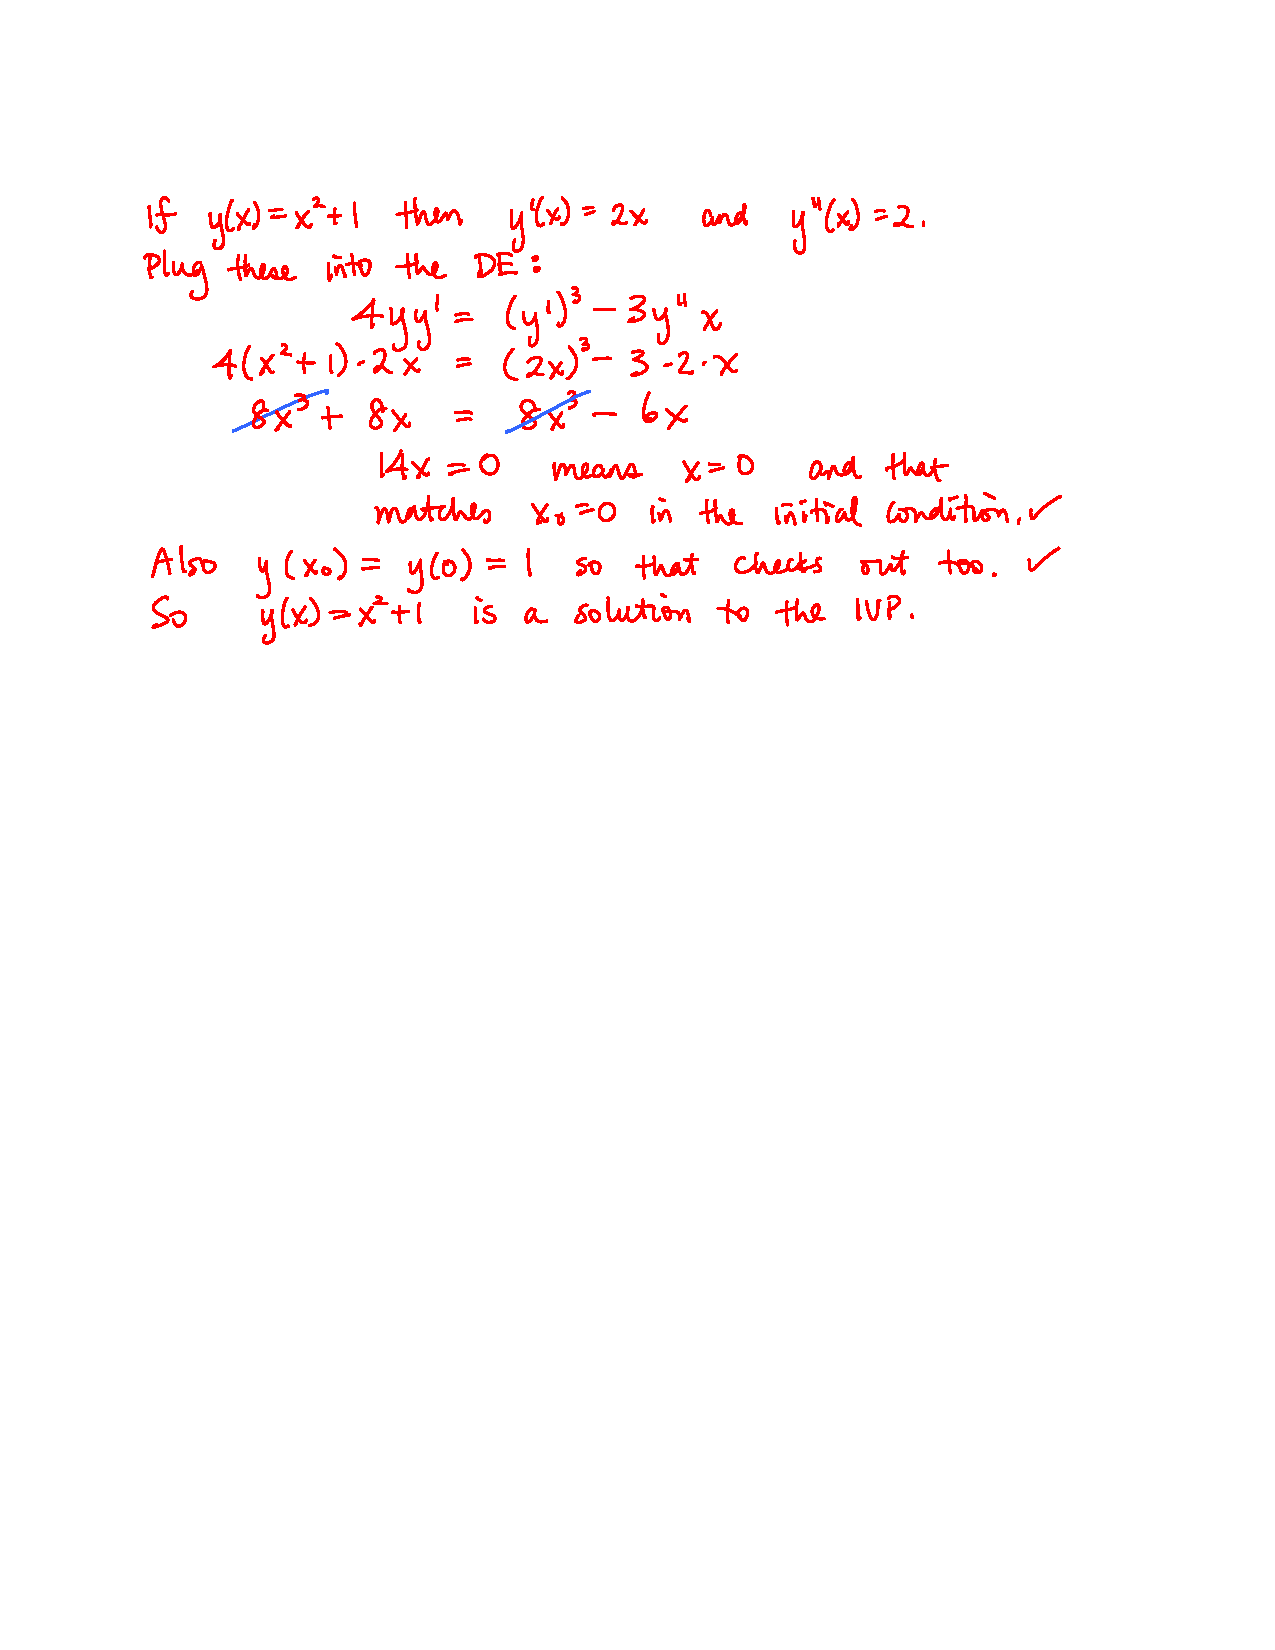
\includegraphics[width=4.5in,keepaspectratio=true]{img/mar_8_5}}}
  \end{center}
  \hspace{10pt}
\end{problem}

\begin{solution}
\vfill
\end{solution}
\newpage

\end{document}
